\documentclass[]{exam}
\usepackage{amssymb}
\usepackage{amsfonts}
\usepackage{amsmath}
\usepackage{amsthm}
\usepackage[top=1in, bottom=1.5in, left=1in, right=1in]{geometry}
\usepackage{tikz}
\usepackage{pgfplots}
\usepackage{empheq}
\usepackage{mathrsfs}
\checkboxchar{$\Box$}
\usepackage{graphicx}
\usepackage{caption}
\usepackage{float}
\usepackage{enumerate}
\usepackage{comment}
\usepackage{multicol}
\usepackage{color}
\usepackage{advdate}
\usepackage{gensymb}
\usetikzlibrary{arrows}
\usepackage{multirow}
\usepackage{arydshln}
\usepackage{verbatim}
\usepackage{lastpage} 
\usepackage{extramarks}
\usepackage{graphicx} 
\usepackage{tikz}
\usepackage{sectsty} 
\usepackage{amsmath,amsfonts,amsthm} 
\usepackage{wrapfig, blindtext}
\usepackage{pgfkeys,pgfcalendar}

\newcount\pgfdatecount
\newcommand{\tomorrow}{%
\pgfcalendardatetojulian{\year-\month-\day+1}{\pgfdatecount}
\pgfcalendarjuliantodate{\the\pgfdatecount}{\myyear}{\mymonth}{\myday}
\pgfcalendarmonthname{\mymonth}\space\myday,\space\myyear%
}

\newcommand{\advanceday}[1][1]{
\begingroup
\AdvanceDate[#1]
\today
\endgroup}

\newcommand{\vertex}{\node[vertex]}
\tikzstyle{vertex}=[circle, draw, inner sep=0pt, minimum size=6pt]

%%%%%%%%%%%%%%%%%%
% Margins
%%%%%%%%%%%%%%%%%%
\topmargin=-0.45in
\evensidemargin=0in
\oddsidemargin=0in
\textwidth=6.5in
\textheight=9.0in
\headsep=0.25in 
\numberwithin{equation}{section}
\linespread{1.1} 
\setlength\parindent{0pt} 
\setlength\answerskip{-.075in}
\setlength\answerlinelength{.5in}
\newcommand{\myitem}{\item[-]}
\pointsinrightmargin
\bracketedpoints

%%%%%%%%%%%%%%%%%%
% HEADER AND FOOTER
%%%%%%%%%%%%%%%%%%
\pagestyle{headandfoot}
\runningheadrule
\runningfootrule
\firstpageheader{Kutztown University}{  }{MATH 210}
\firstpageheadrule
\runningheader{P1.H2}{ }{MATH 210}
\firstpagefooter{}{}{} 
\runningfooter{}{}{Page \thepage\ of \numpages}

%%%%%%%%%%%%%%%%%%
% TITLE PAGE
%%%%%%%%%%%%%%%%%%
\newcommand{\assignmentname}{Phase 1 -- Homework II} 
\newcommand{\coursetitle}{MATH 210 -- Mathematical Computing and Typesetting}
\newcommand{\duedate}{Due: Friday, February 13 by 11:59 PM on D2L} 


\begin{document}
%%%%%%%%%%%%%%%%%%%%%%%%%%%%%%%%%%%%%%%%%%%%%%%%%%%%%
% COMPILE TITLES AND SUCH
%%%%%%%%%%%%%%%%%%%%%%%%%%%%%%%%%%%%%%%%%%%%%%%%%%%%%
\hspace{1in}\\ \vspace{.15in}

\begin{center}
\normalsize
 \fbox{\fbox{\parbox{5.5in}{
        {\bf Instructions:}  Upload the \texttt{tex} file for this document to your Overleaf project.  All solutions shall be completed on this packet by typing your solution in \LaTeX\, in the space provided.  All solutions should be detailed and should clearly demonstrate the process by which you arrived at the answer.  Submit the compiled \texttt{pdf} file to D2L by 11:59 PM on the due date below.  Submit only a single pdf file of your entire packet.  The question will also ask you to make calculations in Python.  Upload any Python files to the appropriate folder in your GitHub repository.  In this folder, a \texttt{py} file is to be submitted for each problem such that when the \texttt{py} file is executed, the output (as presented in Python) is the solution to the problem. Academic dishonesty will not be tolerated.  }}}
\end{center}

\vspace{.5cm}

\begin{center}
	\Huge\textsc{
	\assignmentname}\\[4pt]
        \Large{\textsc{\coursetitle}\\[10pt]}
        \Large{\textsc{\duedate}\\[8pt]}
\end{center}

\vspace{1cm}

%%%%%%%%%%%%%%%%%%%%%%%%%%%%%%%%%%%%%%
% Uncomment the syntax below when you type up the solutions and type 
% your name.
\begin{center}
	\large{\textsc{\textcolor{red}{Solutions by Brooks Emerick}}}
\end{center}
\vfill

%%%%%%%%%%%%%%%%%%%%%%%%%%%%%%%%%%%%%%
% Reminders:
%%%%%%%%%%%%%%%%%%%%%%%%%%%%%%%%%%%%%%
Remember to begin your \texttt{py} file with \texttt{import numpy as np} and \verb|import matplotlib.pyplot as plt|.  



% Blank Page
\clearpage

\begin{questions}
%%%%%%%%%%%%%%%%%%%%%%%%%%%%%%%%%%%%%%
% NUMBER 1 
%%%%%%%%%%%%%%%%%%%%%%%%%%%%%%%%%%%%%%
\question Stokes' Theorem is written so eloquently in my handwriting below.  Replace the figure below with a typed out version of the theorem.  Here are some commands you may need: \verb|\nabla|, \verb|\cdot|, \verb|\partial|, \verb|\Omega|, \verb|\sigma|, \verb|\oint|, among others.  Also, when typing vectors, the symbols are bolded and do not need the little arrow on top, use \verb|\boldsymbol{}|. \\ 

\textsc{Solution:} \\

\underline{Stokes' Theorem:} Let $\Omega$ be an orientable piecewise-smooth surface that is bounded by a simple, closed, piecewise-smooth boundary curve $\partial \Omega$ with positive orientation.  Let $\boldsymbol{F}$ be a vector field whose components have continuous partial derivatives on an open region in $\mathbb{R}^3$ that contains $\Omega$.  Then 

\[ \oint_{\partial \Omega} \boldsymbol{F} \cdot \boldsymbol{T}\, ds = \iint_{\Omega} \left( \nabla \times \boldsymbol{F}\right) \cdot d\boldsymbol{\sigma}. \]



\pagebreak

%%%%%%%%%%%%%%%%%%%%%%%%%%%%%%%%%%%%%%
% NUMBER 2
%%%%%%%%%%%%%%%%%%%%%%%%%%%%%%%%%%%%%%
\question Suppose we're trying to maximize the volume of a squared-based box.  In part $a$, we must supply all sides of the box.  In parts $b$ and $c$, there exists natural borders where we do not need to supply certain sides of the box.  Summarize the three cases below for maximizing volume, $V$, given the surface area, $A$.  For each case, provide the optimal dimensions, $x$ and $y$, and the maximum volume, $V_{max}$, all of which should be a function of $A$.  Create a Python code that will produce a graph with three curves on it, where each curve is $V_{max}$ versus $A$ for each case below.  The legend should decipher each part.  Include the figure in your write-up below.  


\begin{center}
	\includegraphics[width = \textwidth]{P1_HW2_Figure_2.png}
\end{center}

\textsc{Solution:}  The three parts to this problem can be solved simultaneously by introducing a parameter that represents the number of sides that are occupied by walls.  Let $n$ be a value from the set $\{0, 1, 2\}$, then the surface area constraint of this problem can be generalized to the following equation: 
\[ (4-n)xy + 2x^2 = A \qquad \Rightarrow \qquad y = \frac{1}{4-n} \left(\frac{A}{x} - 2x \right). \]
Here, $n = 0$ corresponds to part $a$, $n = 1$ corresponds to part $b$, and $n = 2$ corresponds to part $c$.  In each case,we wish to maximize the volume, $V = x^2y$.  Substituting $y$ into this equation gives the single variable function
\[ V(x) = x^2 \left[ \frac{1}{4-n} \left(\frac{A}{x} - 2x \right) \right] \qquad \Rightarrow \qquad V(x) = \frac{1}{4-n} \left(Ax - 2x^3\right). \]

This function has a unique global minimum value at the critical point that satisfies $V'(x) = 0$: 
\[\frac{1}{4-n} \left( A - 6x^2\right) = 0 \qquad \Rightarrow \qquad x_{max} = \sqrt{\frac{A}{6}}. \]
We note here that the optimal length of the square base doesn't depend on $n$.  However, the height, given by $y$, does depend on $n$: 
\begin{align*}
y_{max} & =  \frac{1}{4-n} \left(\frac{A}{x_{max}} - 2x_{max} \right) \\ 
& =  \frac{1}{4-n} \left(\frac{A}{\sqrt{\frac{A}{6}}} - 2\sqrt{\frac{A}{6}}\right) \\ 
& = \frac{1}{4-n} \left( \sqrt{6}\sqrt{A} - \frac{2}{\sqrt{6}} \sqrt{A} \right)\\
& = \frac{1}{4-n} \left( \frac{6}{\sqrt{6}} - \frac{2}{\sqrt{6}}\right) \sqrt{A}\\
& = \frac{4}{4-n}\sqrt{\frac{A}{6}} \end{align*} 

Finally, using the optimal dimensions for $x$ and $y$ above, we can formulate an expression for the maximal volume: 
\[ V_{max} = \left(\sqrt{\frac{A}{6}}\right)^2\left(\frac{4}{4-n} \sqrt{\frac{A}{6}}\right) \qquad \Rightarrow\qquad V_{max} = \frac{4}{4-n}\left( \frac{A}{6}\right)^{3/2}. \]

Ultimately, we find that the square base always has the same length for any number of sides taken away.  However, the height of the box will grow with $n$, doubling in size when $n$ changes from $0$ to $2$.  Likewise, the optimal volume increases with $n$ and will double in size when $n$ changes from $0$ to $2$.  Figure \ref{Max_Volume_Graph} depicts each part below and shows how the maximum volume, $V_{max}$, changes with surface area, $A$. 

\begin{figure}[h!]
\begin{center}
	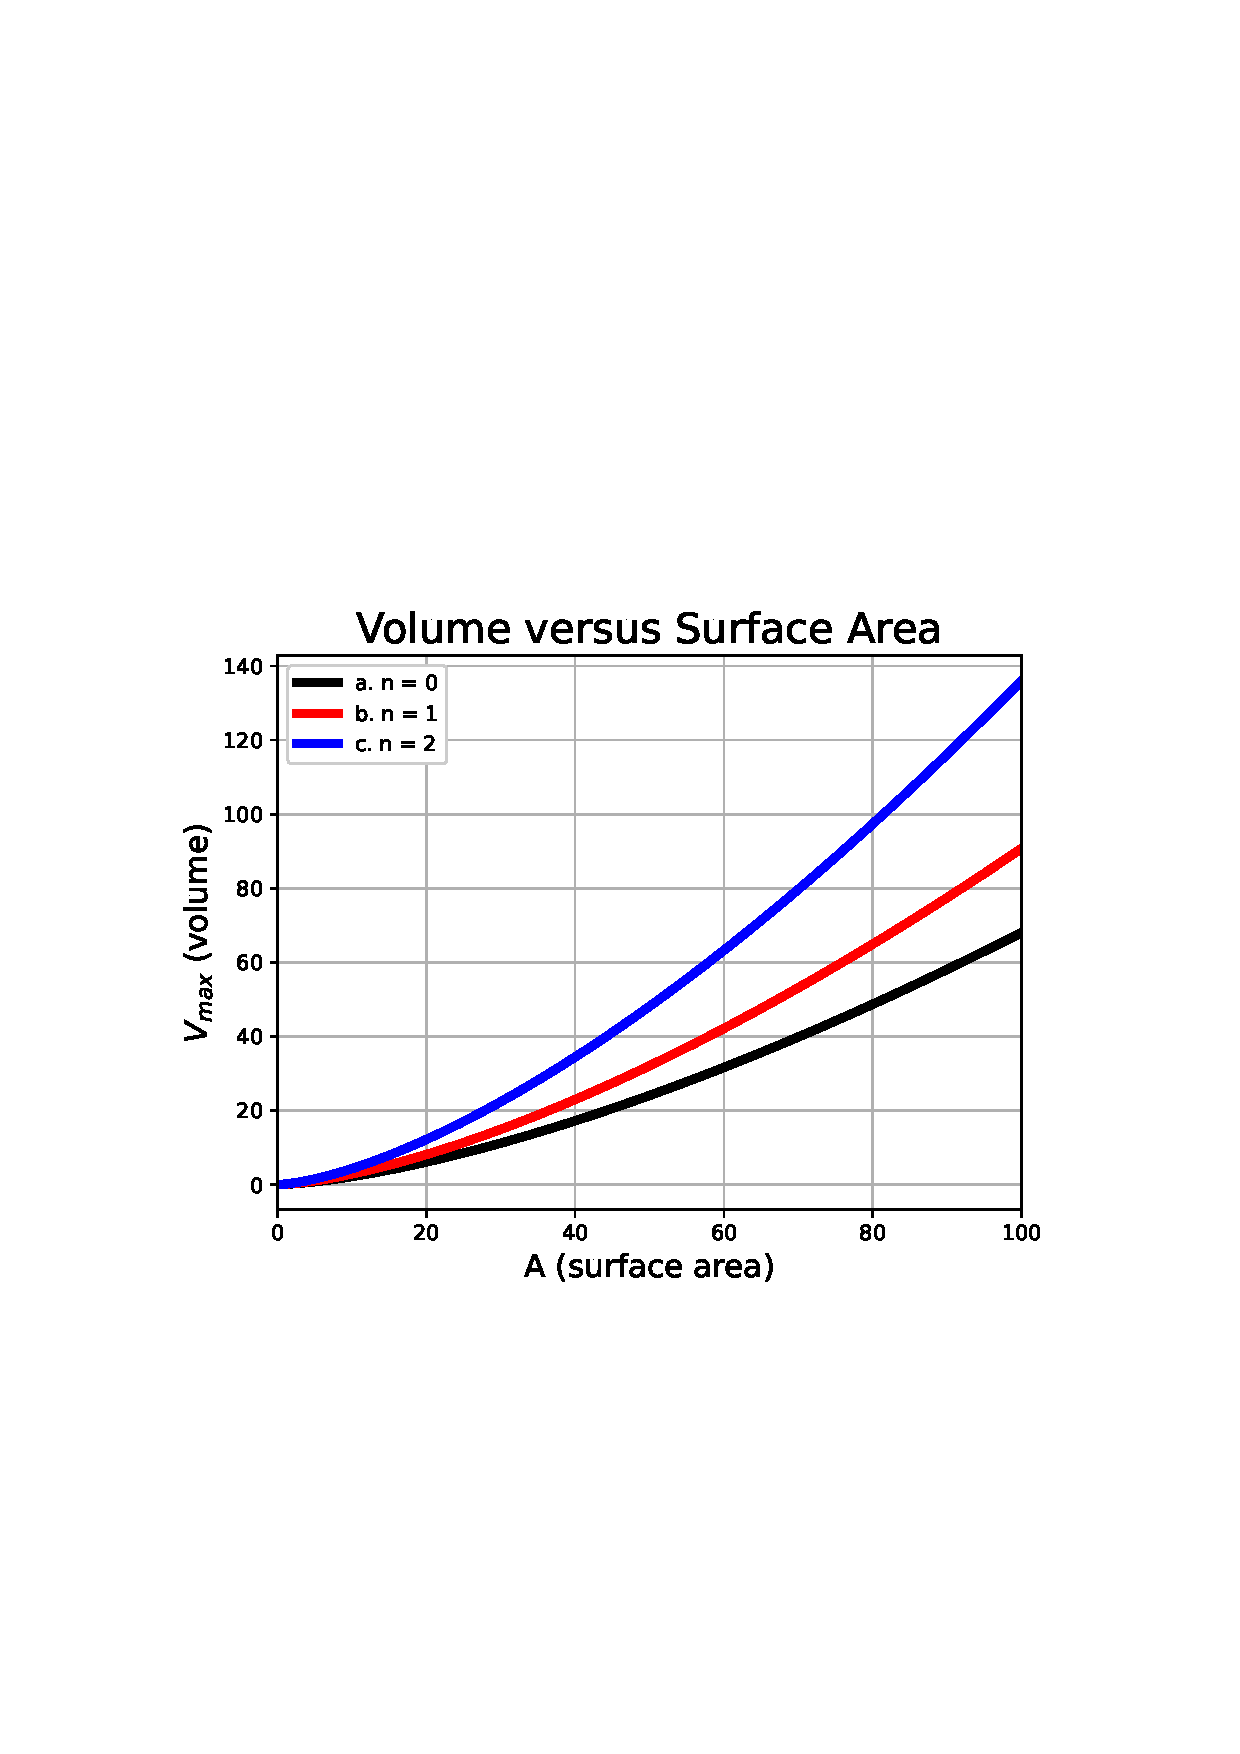
\includegraphics[width = .8\textwidth]{p1hw2_plot1.png} 
\caption{Optimal volume denoted by $V_{max}$ as it relates to surface area, $A$.  We can see that as $n$ increases, the maximum volume increases more rapidly with $A$, indicating that for any given surface area, the volume contained is larger when walls are used as sides. }
\label{Max_Volume_Graph}
\end{center}
\end{figure}




\pagebreak

%%%%%%%%%%%%%%%%%%%%%%%%%%%%%%%%%%%%%%
% NUMBER 3
%%%%%%%%%%%%%%%%%%%%%%%%%%%%%%%%%%%%%%
\question Consider the object below that consists of a cylinder with a spherical cap and a reinforced ``ring" around where the cylinder connects to the hemisphere.  The cost of this ring is $\$c/\text{in}$, the cost of the material to create the cylindrical side and bottom is $\$c_b/\text{in}^2$, and the spherical cap costs $\$c_t/\text{in}^2$.  We want to construct this object that has volume $V$ with the minimal cost.  Construct a cost function, $f$, that is dependent on $r$, the radius of the sphere and cylinder.  Your answer should also be dependent on the parameters $c$, $c_t$, $c_b$, $V$.  Find the value of $r$ that will minimize cost given any set of parameter values.  Create a Python file that will build the function $f$ and find the critical point $r$ that yields the least cost given any values of the parameters.  (No figure is needed, your Python file should print out the value of $r$ for any supplied values of $c$, $c_t$, $c_b$, and $V$.) 

\begin{center}
	\includegraphics[width = .5\textwidth]{P1_HW2_Figure_3.png}
\end{center}

\textsc{Solution:} The object consists of a cylinder and a hemisphere.  The volume of a cylinder is $\pi r^2 h$ and the volume of a hemisphere is $\frac{2}{3}\pi r^3$.  Therefore, our volume constraint can be used to eliminate the variable $h$: 
\[ \pi r^2 h + \frac{2}{3}\pi r^3 = V \qquad \Rightarrow \qquad h = \frac{V}{\pi r^2} - \frac{2}{3}r.\]
Here, $V$ will act as an input to the system and will join $c, c_t$, and $c_b$ as a parameter.  The total cost of the object is the objective function and depends on the costs of the top hemisphere, the cylindrical siding, bottom circle, and the reinforced ring: 
\[ \text{Total Cost:}\,\, c_b(\pi r^2) + c_b(2\pi r h) + c_t(2\pi r^2) + c(2\pi r). \]
Substituting in our expression for $h$ gives our cost function as 
\begin{align*}
f(r) & = c_b\pi r^2 + 2c_b \pi r \left(\frac{V}{\pi r^2} - \frac{2}{3}r \right) + 2c_t \pi r^2 + 2c \pi r \\ 
\qquad \Rightarrow \quad f(r) & = \left( 2c_t - \frac{1}{3} c_b\right) \pi r^2 + 2c\pi r + \frac{2c_b V}{r} \end{align*}

Given any values of $c, c_t, c_b$, and $V$, this function has a unique minimum value on $r\in(0,\infty)$, provided that the first coefficient is positive, i.e. 
\[ 2c_t - \frac{1}{3}c_b > 0 \qquad \Rightarrow \qquad \frac{c_b}{c_t} < 6, \]
which requires that the cost ratio between the bottom and the top must no more than $6$ to $1$.  That is, if the bottom cost more than 6 times the cost of the top, the cost function does not have a unique minimum value for positive $r$.  In this case, the function may attain both a relative minimum and relative maximum. Assuming the inequality above is achieved, the minimum value occurs at the root of $f'(r)$: 
\[ 2\left( 2c_t - \frac{1}{3} c_b\right) \pi r + 2c\pi - \frac{2c_b V}{r^2} = 0 \qquad \Rightarrow \qquad  2\left( 2c_t - \frac{1}{3} c_b\right) \pi r^3 + 2c\pi r^2 - 2c_b V = 0 , \]
which we can solve for numerically in Python. 



\pagebreak





\end{questions}
\end{document} 
